\subsection{Operator Product Expansion}

%The most pessimistic solution to the flavour problem is Minimal Flavour Violation (MFV)
%which simply assumes that beyond SM physics follows a Yukawa coupling like structure in the flavour
%sector, this would lead to no discernible new physics in the flavour sector.

Effective field theories are based on the premise that they processes are defined by the typical
energy scale, $\mu$, at which they operate.
Contributions from particles with very high mass, much greater than $\mu$ are suppressed.
An equally valid interpretation is that massive, unstable particles have short lifetimes and can
only interact over very small distances.
Processes operating at different energy scales are separated both spatially and temporally; and are
therefore decoupled.

Effective field theories allow processes to be modelled at a scale relevant to the particles
involved.
This is often applied to weak interactions of the \bquark quark.
Instead of calculating \bquark decays using the full range of processes outlined by the SM, the
particles who contribute at scales above $m_\bquark$ are integrated out, above a scale $\Lambda$,
leaving the physics that is most relevant at the scale $\mu\simeq m_\bquark$.
Here, processes are dominated by QCD, but higher scale effects still contribute.
A canonical example of this is Fermi's effective theory of weak decays which predates electroweak
theory; in it, a process (such as $\beta$-decay) is collapsed into a four point interaction.


The most general way to parameterize the full effective theory is with an effective Hamiltonian
describing generic
interactions at an energy scale $\mu$, in which long and short distance effects are separated.
Long distance (equivalently low energy) effects are described by coefficients, $c$, which can be
calculated using perturbative methods.
Short distance (or high energy) effects are characterized by terms of operators, $\mathcal{O}$,
which must be calculated non-peturbatively because they contain QCD interactions.
The resulting effective Hamiltonian includes a sum over all processes, $i$, which contribute at a
given dimension, $d$:
\begin{equation}
  \bra{f}\Ham{full}\ket{i} =
  \left.\sum_{d}\frac{1}{\Lambda^{d-4}}
  \sum_i c_i^{(d)}\bra{f}\Op{i}^{(d)}\ket{i}\right|_{\Lambda}.
\end{equation}




%The effective Hamiltonian for the FCNC $\decay{b}{s\ell^+\ell^-}$ is given by:
%\begin{equation}
  %\Ham{eff} = -4\frac{G_F}{\sqrt{2}}\Vconj{ts}\V{tb}\frac{e^2}{16\pi^2}
  %\sum_{i}\big(c_i(\mu)\mathcal{O}_i(\mu)+c_i(\mu)^\prime\mathcal{O}_i^\prime(\mu)\big)
%\end{equation}
%similar to \Eq{eq:th:lageff}, where the coefficients are known as Wilson coefficients, which
%correspond to the Wilson operators $\mathcal{O}_{1-10}$.
%The operators $\mathcal{O}_{1-6}$ are sensitive to long distance contributions such as \ccbar
%loops.
%Operators which are particularly sensitive to NP contributions in \decay{b}{s\mumu} transitions are
%\begin{align}
  %\Op{7\pz} &= \frac{m_b}{e}\big(\bar s \sigma_{\mu\nu}P_Rb\big)F^{\mu\nu}
  %&\Op{7\pz}^\prime &= \frac{m_b}{e}\big(\bar s \sigma_{\mu\nu}P_Lb\big)F^{\mu\nu}
  %\nonumber\\
  %%\mathcal{O}_8 &= g\frac{m_b}{e^2}\big(\bar s \sigma_{\mu\nu}T^aP_Rb\big)G^{\mu\nu a}
  %%&\mathcal{O}_8^\prime &= g\frac{m_b}{e^2}\big(\bar s \sigma_{\mu\nu}T^aP_Rb\big)G^{\mu\nu a}
  %%\\
  %\Op{9\pz} &= \big(\bar s\gamma_\mu P_Lb\big)\big(\bar\ell\gamma^\mu\ell\big)
  %&\Op{9\pz}^\prime &= \big(\bar s\gamma_\mu P_Rb\big)\big(\bar\ell\gamma^\mu\ell\big)
  %\nonumber\\
  %\Op{10} &= \big(\bar s\gamma_\mu P_Lb\big)\big(\bar\ell\gamma^\mu\gamma_5\ell\big)
  %&\Op{10}^\prime &= \big(\bar s\gamma_\mu P_Rb\big)\big(\bar\ell\gamma^\mu\gamma_5\ell\big)
  %\phantom{\frac{1}{1}}
  %%\\
  %%\mathcal{O}_{S} &= \frac{m_b}{m_{B_s}}\big(\bar s\gamma_\mu P_Rb\big)\big(\bar\ell\ell\big)
  %%\\
  %%\mathcal{O}_{P} &= \frac{m_b}{m_{B_s}}\big(\bar s\gamma_\mu P_Rb\big)\big(\bar\ell\gamma_5\ell\big)
%\end{align}
%where $P_{L,R}$ are the left and right projection operators.
%The operators \Op{7} and \Op{9} describe the emission of a photon or $Z$ from a penguin loop,
%and \Op{10} corresponds to a box type diagram with \Wp; these are shown in \Fig{fig:hhh:loops}.
%Primed operators are the suppressed helicity, whose contributions are vanishingly small in the SM.

%\begin{figure}
  %\begin{center}
    %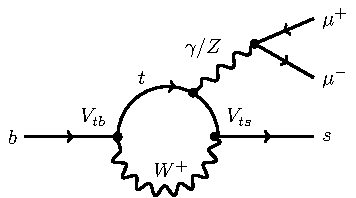
\includegraphics[scale=1]{feynman_btosmumu_penguin}
    %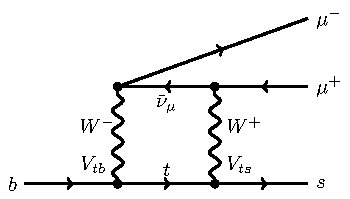
\includegraphics[scale=1]{feynman_btosmumu_box}
    %\caption[Schematic Feynman diagrams for loop and box diagrams]
    %{\small
      %Schematic Feynman diagrams for the
      %(left) penguin loop diagrams corresponding to the operators \Op{7} and \Op{9} depending on
      %whether a $\gamma$ or $Z$ is emitted from the loop;
      %(right) \Op{10} box diagram mediated by \Wp bosons.
    %}
    %\label{fig:hhh:loops}
  %\end{center}
%\end{figure}

%As well as in loops, virtual particles can also contribute in some tree level diagrams.
%The small value of $|\V{ub}|$ means that annihilation decays of \Bp mesons are heavily
%suppressed in the SM.
%%They are mediated by
%%Tree level diagrams in the SM are typically high statistics modes, however annihilation type decays
%%are heavily suppressed.
%These rare modes are propagated by a \Wp in the SM; but this could be exchanged for any charged
%boson, such as an $H^+$ from SUSY, this could alter the branching fraction or
%introduce significant CPV.
%%The decay \btodsphi is an annihilation decay of the \Bp.

%New physics models must be able to accommodate Dark Matter.
%Some models have a \emph{dark} or \emph{hidden} sector which, apart from gravity, only
%communicates with the visible sector feebly via messenger particles.
%These messenger particles could potentially be observed after they decay into SM particles after
%mixing with a $H$ or $Z$.
%The axion could be such a particle, as could the inflaton or dark $Z$; models including these
%particles are further detailed in \Sec{sec:db:intro}.
%
%%Dark Matter is the lightest supersymmetric particle which is stable and messenger particle is super
%%goldstino
%Supersymmetry (SUSY) is a theory which introduces an additional super-particle for each SM fermion and
%gauge boson, whose spin is different by a half integer.
%The Higgs sector in SUSY comprises four Higgs doublets; two are spin-0 and two are spin-$\tfrac12$,
%and then there are two each for $Y=\pm\tfrac12$.
%After SUSY is broken there are five Higgs physical scalar particles, two are CP-even ($h^0$,
%$H^0$) one is CP-odd scalar ($A^0$) and two charged are charged ($H^\pm$).
%Supersymmetry supplies a Dark Matter candidate in the shape of the lightest supersymmetric
%particle, which could communicate with the visible sector via a super-golstino.
%It also immediately solves the hierarchy problem.
%The masses of the super-particles are unconstrained, and could be anywhere between a few TeV and
%the Planck scale.
%%The theory of SUSY immediately solves the hierarcy problem and provide a candidate for Dark Matter
%%in the shape of the lightest supersymmetric particle.
%%Super-goldstino
%%The messenger particles are super goldtinos that arise from the breaking of the symmetry,
%%However, the scale of the masses of the new particles are undefined, meaning
%%they could appear anywhere from a few TeV up to the Planck scale.
%
%
%The most pessimistic solution to the flavour problem is Minimal Flavour Violation (MFV)
%which simply assumes that beyond SM physics follows a Yukawa coupling like structure in the flavour
%sector, this would lead to no discernible new physics in the flavour sector.
%Assuming that nature has not chosen MFV, then contradictions from flavour problem indicate that NP
%searches should be made for both: particles
%with high mass, and particles which have small coupling strengths.
%The \lhcb experiment can probe the mass scale, since precision measurements of tree and loop
%diagrams are sensitive to virtual particles contributing at all orders, whose on-shell mass could
%be many TeV.
%The relatively high luminosity of interactions supplied by the \lhc mean that \lhcb is also
%sensitive to low coupling strengths, such as messenger particles from the dark sector.
%The following chapters explore a variety of different searches for beyond Standard Model physics.
%


